\section{Zusammenfassung und Diskussion}

In Versuch 222 setzten wir uns mit dem Heißluft- bzw. Stirlingmotor auseinander. Dieser wurde im Jahr 1816 von Robert Stirling zum Patent angemeldet. Die Funktionsweise des Heißluftmotors basiert auf einem thermodynamischen Kreisprozess aus abwechselnden isothermen und isochoren Zustandsänderungen, welchen wir im Versuch quantitativ untersuchten.

Im ersten Versuchsteil wurde der Heißluftmotor zunächst nicht als Motor im klassischen Sinne verwendet. Stattdessen trieben wir diesen mit einem externen Motor an, führten also mechanische Arbeit von außen zu. Hierdurch ist es möglich, den eigentlichen Kreisprozess des Motors umzukehren und ihn als Kältemaschine oder auch Wärmepumpe, zur Abkühlung bzw. Aufheizung eines Reservoirs zu verwenden. Die erste Aufgabe war es, die Kälteleistung und Wirkungsgrad der Kältemaschine zu berechnen, sowie die Energiebilanz im System zu untersuchen. Hierzu montierten wir am Zylinder der Kältemaschine eine Heizwendel, mit welcher die entzogene Wärme kompensiert wurde. Anhand der Heizleistung berechneten wir dann die Kälteleistung zu
\begin{align*}
  P_H = (22.29 \pm 0.25) \si{\watt},
\end{align*}
beziehungsweise die Kälteleistung pro Motorumdrehung zu
\begin{align*}
  Q_2 = (4.21 \pm 0.05)\si{\joule},
\end{align*}
was in Relation zur zugeführten mechanischen Arbeit einem Wirkungsgrad von
\begin{align*}
  \eta = 0.440 \pm 0.022
\end{align*}
entsprach. Eine Untersuchung der Energiebilanz zeigte auf, dass dem System im Prozess eine Energie von
\begin{align*}
  \Delta Q = (8.1 \pm 0.7)\si{\joule}
\end{align*}
verloren geht. Diese großen Energieverluste könnten sich auf Wärmeverluste durch unzureichende Isolation, mechanische Reibung, ineffiziente Energieübertragung und Verluste im Kühlkreislauf zurückführen lassen. Zusätzlich könnten Messfehler oder Unsicherheiten sowie das nicht-ideale Verhalten des realen Stirlingprozesses, dies zeigt sich durch die abgerundeten Isochoren, eine Rolle spielen. Auch Effizienzverluste des Elektromotors bei der Umwandlung von elektrischer Energie zu mechanischer Arbeit können Gründe für die Abweichungen sein.

Für den zweiten Versuchsteil trieben wir den Heißluftmotor weiterhin extern an. Anstelle der Heizwendel montierten wir nun ein Reagenzglas mit Wasser am Motor. Wir betrieben diesen zunächst erneut als Kältemaschine, um das Wasser auf etwa $-30\si{\celsius}$ herunterzukühlen und anschließend als Wärmepumpe um das Wasser wieder aufzuheizen, bis es in etwa $100\si{\celsius}$ erreichte. Über den kompletten Vorgang hinweg zeichneten wir die Wassertemperatur auf. Eine detaillierte Interpretation des Temperaturverlaufs ist im entsprechenden Abschnitt der Ausarbeitung zu finden. \abbref{fig:tempverlauf_unter0} zeigt noch einmal den interessantesten Teil des Temperaturverlaufs um und unter der $0\si{\celsius}$-Marke.

\begin{figure}[H]
  \centering
  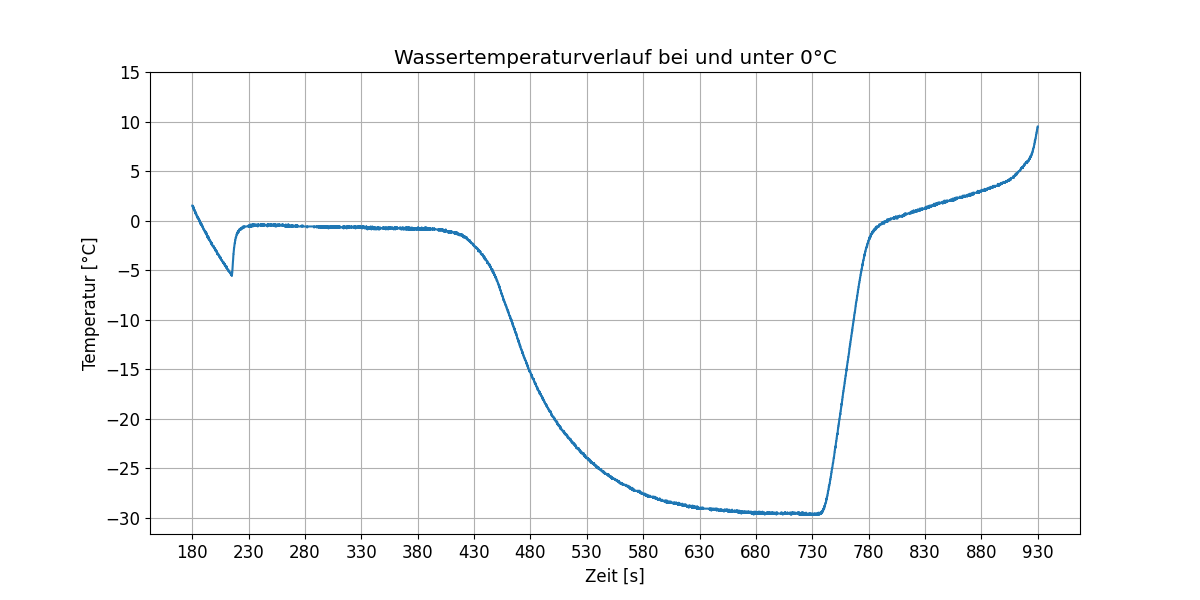
\includegraphics[width=.9\textwidth]{files/tempverlauf_unter0.png}
  \caption{Wassertemperaturverlauf beim Betrieb als Kältemaschine und Wärmepumpe für etwa $1 \si{\milli\liter}$ Wasser um und unter $0\si{\celsius}$.}
  \label{fig:tempverlauf_unter0}
\end{figure}

Besonderes Augenmerk legten wir hierbei auf den Plateaubereich, der sich ab etwa Sekunde $230$ einstellte. In dieser Zeit wurde nahezu alle Energie für den Phasenübergang des Wassers zu Eis benötigt, weshalb es hier nicht weiter abgekühlt wird. Aus der Länge dieses Plateaus konnten wir anhand der spezifischen Schmelzwärme von Wasser erneut die Kälteleistung der Kältemaschine berechnen. Hierbei kamen wir auf einen Wert von
\begin{align*}
  P_G = (1.856 \pm 0.021)\si{\joule\per\second}.
\end{align*}
Diese Kühlleistung ist sehr viel geringer, als die zuvor mittels der Kompensationsmessung bestimmte Kühlleistung. Ursachen dafür könnten wie folgt aussehen. In Abschnitt 3.1 maßen wir den Strom und die Spannung, welche Heizwendel anliegen, um daraus die Heizleistung zu bestimmen. Hierbei sind wir davon ausgegangen, dass die Umwandlung von elektrischer Energie zu Wärme ideal abläuft, was in Realität nicht der Fall ist. Weiter beziehen die Berechnungen in 3.1 die Kompensation aller Wärmeverluste des Systems mit ein. Dies sind neben dem tatsächlichen Wärmeentzug durch die Kältemaschine auch die bereits erwähnte Verluste durch unzureichende Isolation und Abstrahlung. Im zweiten Versuchsteil betrachteten wir über die Temperaturmessung ausschließlich die notwendige Energie für den Phasenübergang.

In Versuchsteil drei beschäftigen wir uns mit der Umwandlung von zugeführter Wärme in mechanische Arbeit. Hierzu brachten wir wieder die Heizwendel am Zylinder des Motors an. In einer Leerlaufmessung bestimmten wir zunächst die zugeführte elektrische Leistung und Wärme, die an das Kühlsystem abgeführte Wärme, sowie die vom Motor aufgebrachte mechanische Arbeit. Für letzteres zeichneten wir mit der Software \textit{Cassy Lab} das $pV$-Diagramm des Kreisprozesses auf und berechneten die mechanische Arbeit aus dessen Fläche. Als Verhältnis der mechanischen Arbeit zur zugeführten elektrischen Energie bestimmten wir den thermischen Wirkungsgrad zu
\begin{align*}
  \eta_{th} = 0.0517 \pm 0.0007.
\end{align*}
Dieser ist sehr gering, was sich auch in den sehr hohen Verlusten in einer Höhe von
\begin{align*}
    Q_V = 16.6 \pm 0.6 \si{\joule}
\end{align*}
durch Wärmeabstrahlung, Wärmeleitung und Reibung widerspiegelt. Die Gründe für die Höhe der Verluste sind größtenteils dieselben, wie sie auch bereits zu den vorherigen Versuchsteilen genannt wurden. Deshalb werden wir an dieser Stelle nicht noch einmal näher auf diese eingehen.

Für den zweiten Abschnitt des dritten Versuchsteils brachten wir an der Antriebswelle des Heißluftmotors einen Bremszaum an, welcher mit einem Federkraftmesser verbunden war. Für vier unterschiedliche Einstellungen der Bremskraft ermittelten wir die vom Motor ausgeübten Drehmomente. Diese nutzten wir, neben der Fläche des $pV$-Diagramms, als eine weitere Weise, die verrichtete mechanische Arbeit des Motors zu berechnen. Als Verhältnis der durch die Drehmomentmessung berechneten mechanischen Arbeit zur zugeführten Wärme berechneten wir in dieser Versuchsreihe unter anderem den effektiven Wirkungsgrad $\eta_{th}$. \tabref{tab:werte_gebremst_kurz} fasst die errechneten Wirkungsgrade zu den eingestellten Bremskräften noch einmal zusammen.

\begin{table}[H]
  \centering
  \begin{tabular}{c c c c c}
  \toprule
  \textbf{Eingestellte Kraft} & \boldmath$f\,\qty[\si{\per\second}]$ & \boldmath$\eta_{\text{th}}$ & \boldmath$\eta_{\text{eff}}$ \\
  \midrule
  \multirow{2}{*}{\boldmath$0.8\si{\newton}$} & $3.194$& $0.0604$ & $0.0277$ \\
   & $\pm 0.012$ & $\pm 0.0007$ & $\pm 0.0008$ \\
  \midrule
  \multirow{2}{*}{\boldmath$0.6\si{\newton}$} & $3.505$ & $0.0617$ & $0.0228$ \\
   & $\pm 0.007$ & $\pm 0.0004$ & $\pm 0.0008$ \\
  \midrule
  \multirow{2}{*}{\boldmath$0.4\si{\newton}$} &  $3.831$& $0.0613$ & $0.0166$ \\
   &  $\pm 0.006$& $\pm 0.0005$ & $\pm 0.0009$ \\
  \midrule
  \multirow{2}{*}{\boldmath$0.2\si{\newton}$} &  $4.245$& $0.0612$ & $0.0092$ \\
   &  $\pm 0.0010$ & $\pm 0.0008$ & $\pm 0.0010$ \\
  \bottomrule
  \end{tabular}
  \label{tab:werte_gebremst_kurz}
  \caption{Berechneter thermischer und effektiver Wirkungsgrad mit Unsicherheiten für verschiedene Bremskrafteinstellungen}
\end{table}
Betrachten wir den funktionalen Verlauf der Wirkungsgrade, auch noch einmal grafisch dargestellt in den Abbildungen (\ref{fig:eta_th_freq}) und (\ref{fig:eta_eff_freq}), fällt auf, dass der thermische Wirkungsgrad, unter Beachtung der großen Fehlerbereiche, weitestgehend konstant bleibt, während der effektive Wirkungsgrad mit steigender Motorfrequenz abfällt. Diese Beobachtungen lassen sich bereits durch die mathematische Betrachtung erklären. Der thermische Wirkungsgrad lässt sich durch Einsetzen auf das Verhältnis $\eta_{th} = \frac{P_{pV}}{P_{el}} \frac{f}{f}$ bringen, hier kürzt sich die Frequenz $f$ also heraus, was die Unabhängigkeit von dieser erklärt. Den effektiven Wirkungsgrad führen wir auf den Bruch $\eta_{eff} = \frac{2 \pi D f}{P_{el}}$ zurück. Wodurch sich die Proportionalität zur Frequenz zeigt.

Die beiden Wirkungsgrade sind unterschiedlich, weil $\eta_{th}$ die gesamte mechanische Arbeit im thermodynamischen Kreisprozess betrachtet, während nur $\eta_{eff}$ die effektiv abgegebene Arbeit am Bremszaum berücksichtigt. Die Diskrepanz resultiert aus Reibungsverlusten, ungenutzter Energie und Ineffizienzen im Motor.